\section{KV-Direct Operation Primitives}
\label{kvdirect:sec:architecture}
\label{kvdirect:sec:kv-operations}

KV-Direct extends the Remote Direct Memory Access (RDMA) primitives to \textit{remote direct key-value access} primitives, as shown in Table \ref{kvdirect:tab:kv-operations}.
The client sends \textit{KV-Direct operations} to the key-value storage server, and the programmable network card processes the requests and sends back the results, bypassing the CPU.
The programmable network card on the key-value storage server is an FPGA reconfigured as a \textit{key-value processor}.

In addition to the standard key-value storage operations shown at the top of Table \ref{kvdirect:tab:kv-operations}, KV-Direct also supports two types of vector operations:
sending a scalar to the network card on the server, the network card will apply the update to each element in the vector; or sending a vector to the server, and the network card updates the original vector element by element.
Furthermore, KV-Direct supports including user-defined functions in atomic operations.
User-defined functions need to be pre-registered and compiled into hardware logic, indexed at runtime using the function ID.
Key-value operations using user-defined functions are similar to \textit{active messages} \cite{eicken1992active}, saving the communication and synchronization costs of retrieving the key-value to the client for processing.

\begin{table}
\centering
\caption{KV-Direct operations.}
\label{kvdirect:tab:kv-operations}
\small
\begin{tabular}{p{.4\textwidth}|p{.5\textwidth} }
\toprule
get ($k$) $\rightarrow v$ & Get the value of key $k$. \\
\midrule
put ($k, v$) $\rightarrow$ bool & Insert or replace the pair $(k, v)$. \\
\midrule
delete ($k$) $\rightarrow$ bool & Delete key $k$. \\
\midrule
\midrule
update{\_}scalar2scalar ($k, \Delta, \lambda(v, \Delta) \rightarrow v$) $\rightarrow v$ & Atomically update key $k$ using function $\lambda$, acting on $\Delta$, returning the original value.\\
\midrule
update{\_}scalar2vector ($k, \Delta, \lambda(v, \Delta) \rightarrow v$) $\rightarrow [v]$ & Atomically update all elements in key $k$ using function $\lambda$ and scalar $\Delta$, returning the original vector. \\
\midrule
update{\_}vector2vector ($k, [\Delta], \lambda(v, \Delta) \rightarrow v$) $\rightarrow [v]$ & Atomically update all elements in key $k$ using function $\lambda$, based on corresponding elements in vector $[\Delta]$, and return the original vector. \\
\midrule
reduce ($k, \Sigma, \lambda(v, \Sigma) \rightarrow \Sigma$) $\rightarrow \Sigma$ & Reduce vector $k$ to a scalar using function $\lambda$, and return the reduced result $\Sigma$. \\
\midrule
filter ($k, \lambda(v) \rightarrow$ bool) $\rightarrow [v]$ & Filter elements in vector $k$ using function $\lambda$, and return the filtered vector. \\
\bottomrule
\end{tabular}
\end{table}

When performing vector operation updates (update), reductions (reduce), or filters (filter) on a key, its value is considered an array of fixed-width elements.
Each function $\lambda$ operates on an element in the vector, client-specified parameter $\Delta$, and/or initial value $\Sigma$ for reduction.
Based on the KV-Direct development toolchain from Chapter \ref{chapter:clicknp}, user-defined function $\lambda$ is replicated multiple times to exploit the parallelism in FPGA and match the computation throughput with the throughput of other components in the key-value processor, then compiled into reconfigurable hardware logic using High-Level Synthesis (HLS) tools \cite{aoc,sdaccel}.
Thanks to the design from Chapter \ref{chapter:clicknp}, the development toolchain automatically extracts data dependencies in the replicated function and generates fully pipelined programmable logic.
Before the key-value storage client starts running, the programmable network card on the key-value storage server should load the hardware logic of user-defined function $\lambda$.

Using user-defined functions, common stream processing can be implemented in vector operations. For example, network processing applications can interpret this vector as a packet stream for network functions, or a set of states for packet transactions \cite {sivaraman2016packet}. It is even possible to implement single-object transaction processing entirely within programmable network cards, such as the operation of resetting S\_QUANTITY to zero after reaching the threshold in the TPC-C benchmark test \cite {council2010tpc}. Vector reduction operations can support the calculation of accumulating neighbor node weights in PageRank \cite {page1999pagerank}. Vector filtering operations can also be used to obtain non-zero values in sparse vectors.

\section{Key-Value Processor}
\label{kvdirect:sec:kv-processor}

\begin{figure}[htbp]
\centering
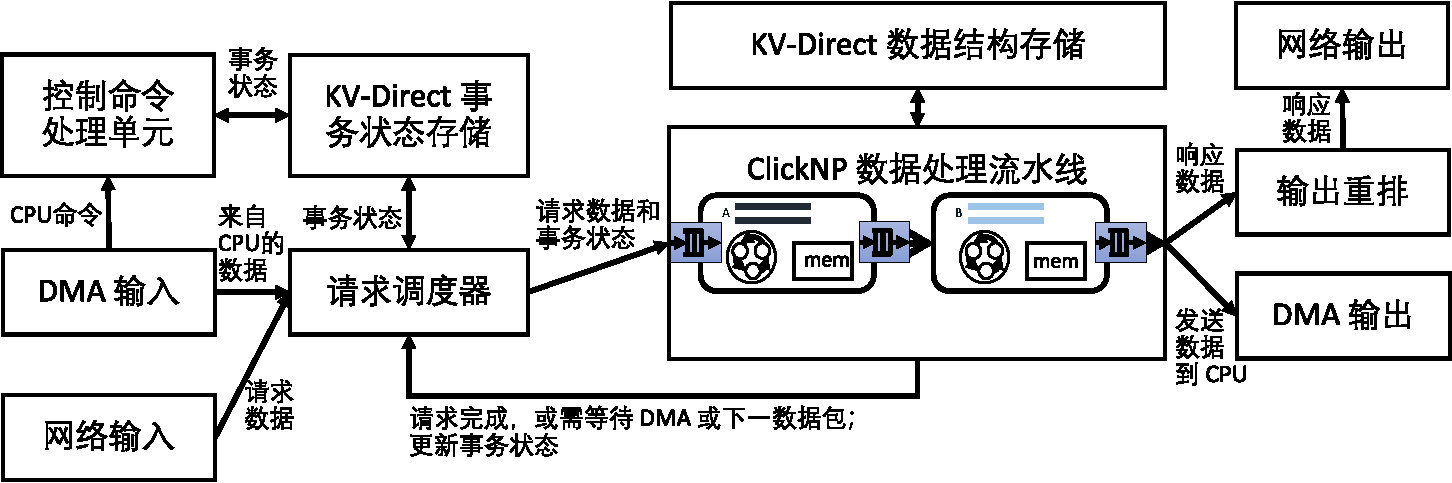
\includegraphics[width=0.6\textwidth]{kvdirect_arch.pdf}
\caption{Architecture of the key-value processor.}
\label{kvdirect:fig:kvprocessor-arch}
\end{figure}

As shown in Figure \ref {kvdirect:fig:kvprocessor-arch}, the key-value processor receives packets from the onboard network card, decodes vector operations, and buffers key-value operations in the reservation station \footnote{The reservation station is a concept in computer architecture that stores operations to be executed and schedules appropriate operations for concurrent execution.} (Section \ref {kvdirect:sec:ooo}). Next, the out-of-order execution engine (Section \ref {kvdirect:sec:ooo}) sends concurrently executable key-value operations from the reservation station to the key-value operation decoder. Depending on the operation type, the key-value processor looks up the hash table (Section \ref {kvdirect:sec:hashtable}) and performs the corresponding operation. To minimize memory access times, smaller key-value pairs are stored inline in the hash table, while other key-value pairs are stored in dynamically allocated memory in the slab memory allocator (Section \ref {kvdirect:sec:slab}). Both the hash index and the memory allocated by the slab are managed by a unified memory access engine (Section \ref {kvdirect:sec:dram-cache}), which accesses the host memory via PCIe DMA and caches part of the host memory in the onboard DRAM. After the key-value operation is completed, the result is sent back to the out-of-order execution engine (Section \ref {kvdirect:sec:ooo}), which looks for key-value operations that depend on it in the reservation station and executes them.

As discussed in Section \ref {kvdirect:sec:challenge}, the scarcity of PCIe throughput requires the key-value processor to save DMA access. For GET operations, at least one memory read is required. For PUT or DELETE operations, for the hash table data structure, at least one read and one write are required \footnote{The read operation takes out the key in the hash slot. If the slot is empty or the same as the key to be searched, and no memory space needs to be reallocated, a write operation is required to write back the data}. Log-based data structures can achieve less than one write operation per PUT on average, but it sacrifices GET performance. KV-Direct carefully designs the hash table to achieve near-ideal DMA access for each lookup and insertion. KV-Direct also carefully designs the memory allocator so that each dynamic memory allocation averages less than 0.1 DMA operations.

\subsection{Hash Table}
\label{kvdirect:sec:hashtable}

To store variable-sized key-values, key-value storage is divided into two parts. The first part is the hash index (Figure \ref {kvdirect:fig:hashtable}), which contains a fixed number of \textit {hash buckets}. Each hash bucket contains several \textit {hash slots} and some metadata. The rest of the memory is dynamically allocated and managed by the slab allocator (Section \ref {kvdirect:sec:slab}). The \textit {hash index ratio} configured at initialization is the proportion of the size of the hash index to the total memory size of the key-value storage. The choice of hash index ratio will be discussed in Section \ref {kvdirect:sec:hashtable-eval}.

\begin{figure}[htbp]
	\centering
	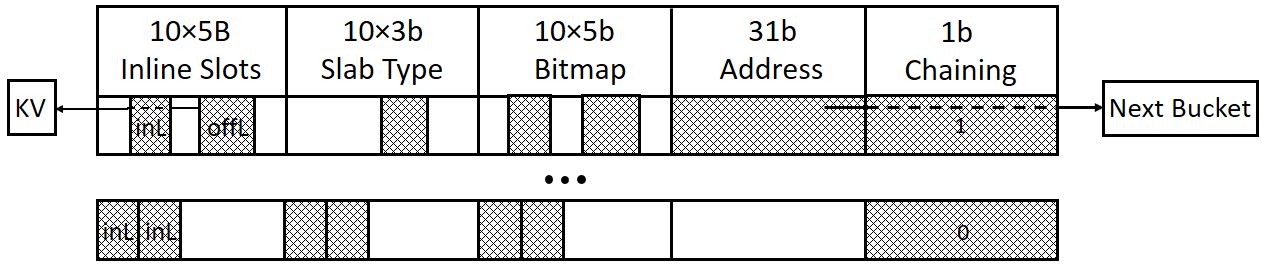
\includegraphics[width=1.0\textwidth,page=1]{hashline.PNG}
	\caption{Hash index structure. Each row is a hash bucket, containing 10 hash slots, each hash slot includes 3 bits of slab memory type, a bitmap marking the start and end of inline key-value pairs, and a pointer to the next linked bucket in case of hash collision.}
	\label{kvdirect:fig:hashtable}
\end{figure}

%\textbf{Hash Table.}
%Each bucket includes 10 hash slots, 3b type code per slot, 50b metadata, plus 31b address and a valid bit of the next chained bucket, as shown in Figure~\ref{kvdirect:fig:hashtable}.
%For offline keys and values, each hash slot needs to store 31b of address, 9b of secondary hash and 3b type code for the slab size.
%For inline keys and values, to mark the begin and end of each hash slot, as well as the separation between inline key and value, the information is encoded in a 50b metadata corresponding to 50 bytes of hash slots.
%The inline keys and secondary hashes of offline keys in all hash slots are compared in parallel, and the first match is found.

Each hash slot includes a pointer to the key-value data in dynamically allocated memory and an \textit{auxiliary hash}. The auxiliary hash is an optimization that uses another hash function independent of the main hash function. Since there are multiple hash slots in each hash bucket, the key-value processor needs to determine which hash slot corresponds to the key to be found. With a 9-bit auxiliary hash, it can be determined with a probability of 511/512 which is the key to be found. However, to ensure correctness, an additional memory access is still needed to fetch the key and compare it byte by byte. Assuming a 64~GiB key-value storage in the host memory and a 32-byte allocation granularity~\footnote{The 32-byte allocation granularity balances the internal fragmentation and the overhead for memory allocation metadata.}, the pointer requires 31 bits. The size of each hash slot is 5 bytes~\footnote{The design parameters in this paper are configured according to the parameters of the hardware platform used in this paper. For memory of different capacities, parameters such as hash slot size and pointer bit width may change.}. To determine the size of the hash bucket, a trade-off needs to be made between the number of hash slots in each bucket and the DMA throughput. Figure \ref{kvdirect:fig:dma-tput} shows that when the granularity is less than 64B, the DMA read throughput is constrained by the PCIe latency and parallelism in the DMA engine. A bucket size less than 64B will increase the possibility of hash collisions. On the other hand, increasing the bucket size to more than 64B will reduce the throughput of hash lookups. Therefore, the bucket size is chosen to be 64 bytes.

The \textit{key-value size} refers to the total size of the key and value. Key-values smaller than the threshold size are stored inline in the hash index to save additional memory accesses to fetch the key-value data. Inline key-values can span multiple hash slots, and their pointer and auxiliary hash fields are reused to store key-value data. Inlining all key-values that can fit into the hash index may not be the best choice. An inline key-value may occupy multiple hash slots, reducing the number of key-values that the hash table can store. If the capacity of the hash table allows, inlining key-values can reduce the average number of memory accesses. For this, KV-Direct selects the \textit{inline threshold} based on the proportion of the hash table that is filled, and inlines key-values smaller than this threshold. Traditionally, the load factor~\footnote{The load factor is the ratio of the number of occupied hash slots to the total number of hash slots.} is used to measure the proportion of the hash table that is filled, but this ignores the overhead brought by the metadata and internal fragmentation of the hash table. To compare the choices of different parameters of the hash table more scientifically, this chapter uses \textit{memory utilization}~\footnote{Memory utilization is the ratio of the sum of the sizes of all key-values in the key-value storage to the total size of the key-value storage. Due to the existence of metadata and internal fragmentation, memory utilization is always less than 1.}. As shown in Figure \ref{kvdirect:fig:inline-offline}, for a certain inline threshold, the average number of memory accesses per key-value operation increases with the increase of memory utilization due to more hash collisions. Under a higher inline threshold, the growth curve of the average number of memory accesses is steeper. Therefore, the optimal inline threshold can be found to minimize the number of memory accesses at a given memory utilization. Like the hash index ratio, the inline threshold can also be configured at initialization.

\begin{figure}[htbp]
	\centering
	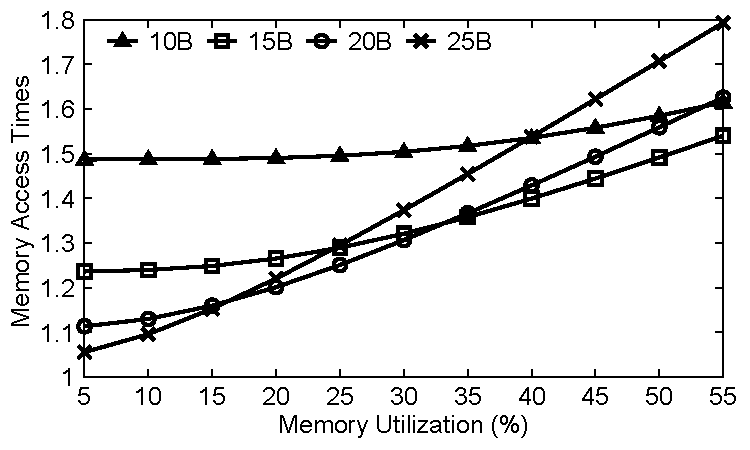
\includegraphics[width=0.6\textwidth]{inline_thresh.pdf}
	\caption{Average number of memory accesses and memory utilization under different inline thresholds.}
	\label{kvdirect:fig:inline-offline}
\end{figure}

When all the hash slots in the hash bucket are filled, there are several solutions to solve the hash collision. Cuckoo Hashing~\cite{pagh2004cuckoo} and Hopscotch Hashing~\cite{herlihy2008hopscotch} ensure that newly inserted key-values are always inserted into the hash bucket by moving occupied hash slots during the insertion process, so that only a constant number of hash slots in the same hash bucket need to be compared during the lookup, achieving constant time lookup. However, in write-intensive workloads, the memory access time under high load rates can fluctuate significantly. In extreme cases, insertion may even fail, requiring hash table expansion. Another solution to hash collisions is \textit{linear probing}, which may be affected by clustering, so its performance is sensitive to the uniformity of the hash function. For this, this paper chooses \textit{chaining} to solve hash collisions, which balances the performance of lookup and insertion, and is more robust to hash clustering.

To compare KV-Direct's chaining, bucketized Cuckoo Hash in MemC3~\cite{fan2013memc3}, and chain associative Hopscotch Hash in FaRM~\cite{dragojevic2014farm}, Figure \ref{kvdirect:fig:mem-access-tput} plots the average number of memory accesses per GET and PUT operation in three possible hash table designs. In the KV-Direct experiment, the best choices are made for the inline threshold and hash index ratio for a given key-value size and memory utilization requirement. In the Cuckoo and Hopscotch hash experiments, it is assumed that the key is inlined and can be compared in parallel, and the value is stored in dynamically allocated slab storage. Since the hash tables of MemC3 and FaRM cannot support a memory utilization rate of more than 55% for a key-value size of 10B (i.e., they have more space occupied by metadata and internal fragmentation), Figure \ref{kvdirect:fig:mem-access-10-get} and Figure \ref{kvdirect:fig:mem-access-10-put} only show the performance of KV-Direct.

\begin{figure}[htbp]
	\centering
	\subfloat[10B GET.\label{kvdirect:fig:mem-access-10-get}]
	{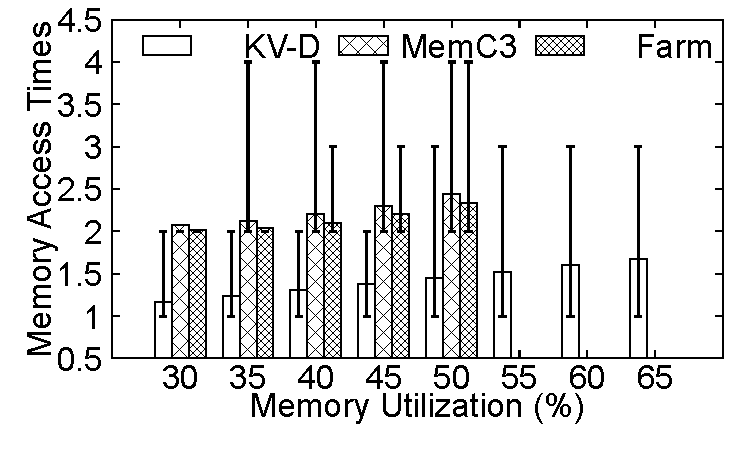
\includegraphics[width=.5\textwidth,page=1]{10B_get.pdf}}
	\subfloat[10B PUT.\label{kvdirect:fig:mem-access-10-put}]
	{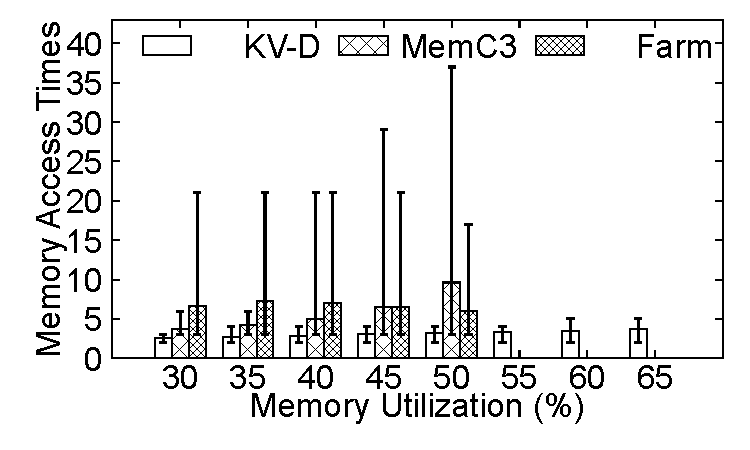
\includegraphics[width=.5\textwidth,page=1]{10B_put.pdf}}
	
	\vfill
	
	\subfloat[254B GET.\label{kvdirect:fig:mem-access-254-get}]
	{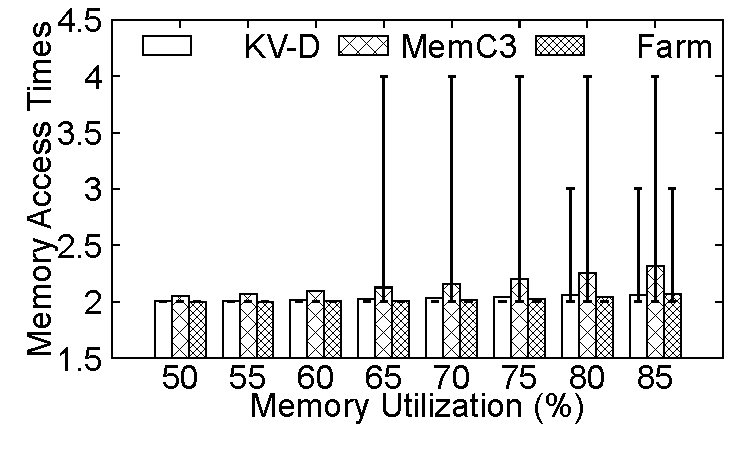
\includegraphics[width=.5\textwidth,page=1]{254B_get.pdf}}
	\subfloat[254B PUT.\label{kvdirect:fig:mem-access-254-put}]
	{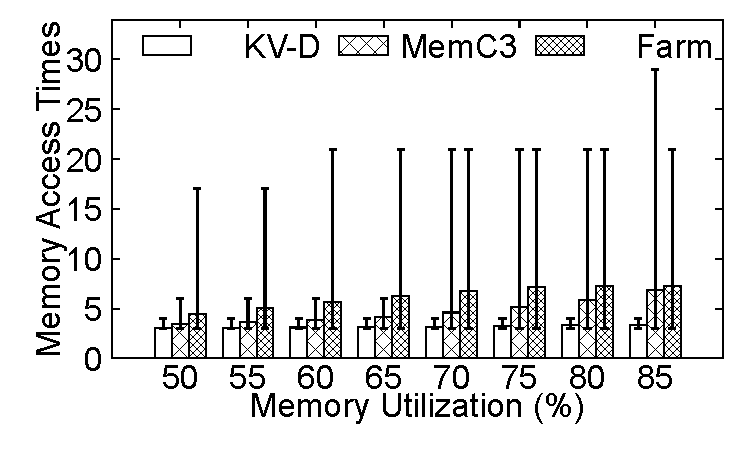
\includegraphics[width=.5\textwidth,page=1]{254B_put.pdf}}
	\caption{Number of memory accesses per key-value operation.}
	\label{kvdirect:fig:mem-access-tput}
\end{figure}

For inline key-values, each GET operation in KV-Direct only requires close to 1 memory access, and each PUT also only requires 2 memory accesses under non-extreme memory utilization. Non-inline key-values have one additional memory access for GET and PUT. Comparing KV-Direct and chained hopscotch hashing under high memory utilization, hopscotch hashing performs better in GET but worse in PUT. Although KV-Direct cannot guarantee the worst-case DMA access times, it will balance between GET and PUT. The GET operation of cuckoo hashing can guarantee access to at most two hash slots, so under most memory utilizations, KV-Direct has more memory accesses. However, under high memory utilization, cuckoo hashing will cause a large fluctuation in the number of memory accesses for PUT operations.

\label{kvdirect:sec:hashtable-eval}

There are two free parameters in the hash table design: (1) inline threshold, (2) the ratio of hash index in the entire memory space. As shown in Figure \ref {kvdirect:fig:optimize_fix_mem}, as the hash index ratio grows, more key-value pairs can be stored inline, resulting in a lower average number of memory accesses. Figure \ref {kvdirect:fig:optimize_fix_ratio} shows the increased number of memory accesses with the use of more memory.

\begin{figure}[htbp]
	\subfloat[Fixed memory utilization 0.5.\label{kvdirect:fig:optimize_fix_mem}]
	{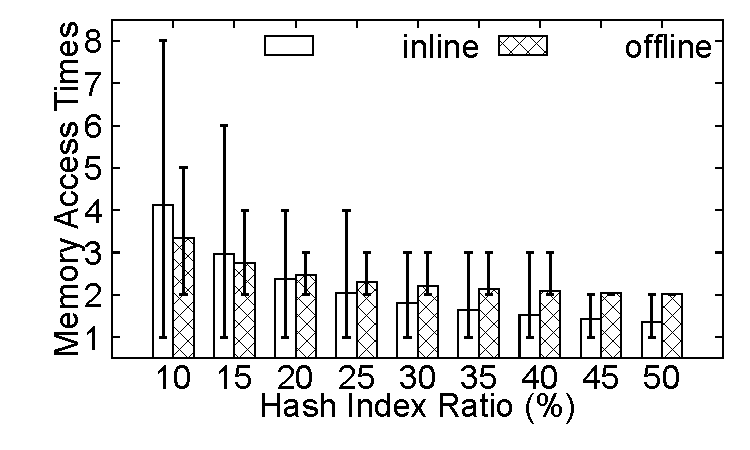
\includegraphics[width=.5\textwidth,page=1]{fix_mem.pdf}}
	\subfloat[Fixed hash index ratio 0.5.\label{kvdirect:fig:optimize_fix_ratio}]
	{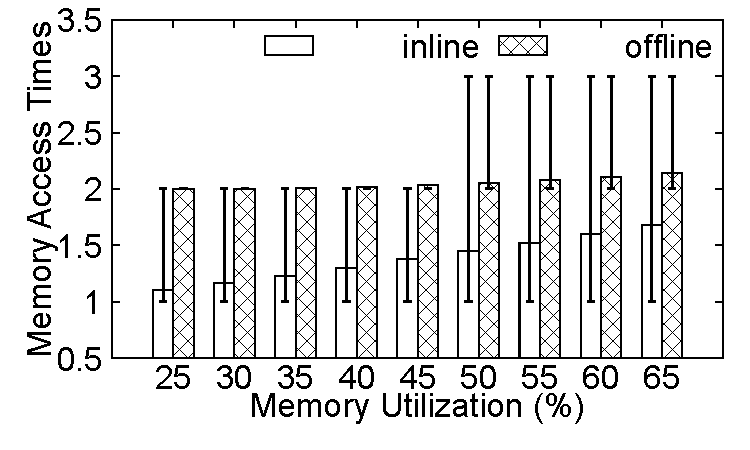
\includegraphics[width=.5\textwidth,page=1]{fix_ratio.pdf}}
	\caption{Memory occupancy at different memory utilization or hash index ratios.}
	\label{kvdirect:fig:memory-access-count}
\end{figure}

As shown in Figure \ref {kvdirect:fig:hashline-ratio}, the maximum memory utilization decreases when the hash index ratio is high, because less memory is available for dynamic allocation. Therefore, to accommodate all key-values to be stored in a given memory space, the hash index ratio has an upper limit. This section chooses this upper limit to obtain the minimum average number of memory accesses, as shown by the dashed line in Figure \ref {kvdirect:fig:hashline-ratio}, first according to the target memory utilization, to get a large hash index ratio; then according to the hash index ratio, the average number of memory accesses required for the GET operation to find the index can be theoretically obtained.

\begin{figure}[htbp]
	\centering
	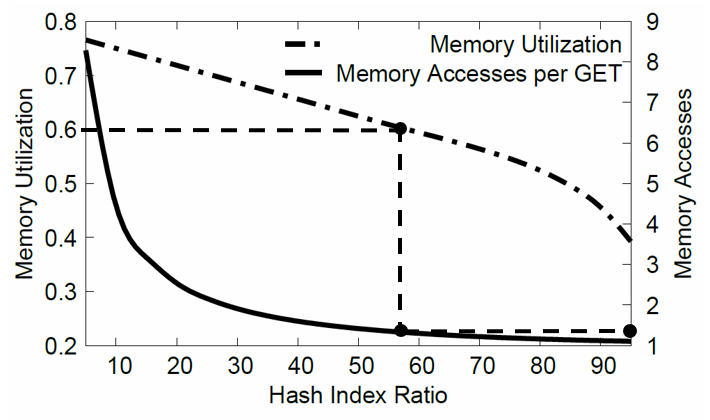
\includegraphics[width=0.6\textwidth,page=1]{optimize.png}
	\caption{How to determine the optimal hash index rate given the memory utilization requirement and key-value size.}
	\label{kvdirect:fig:hashline-ratio}
\end{figure}

\subsection{Slab Memory Allocator}
\label{kvdirect:sec:slab}

Chain hash slots and non-inline key-values require dynamic memory allocation. For this, this chapter chooses the slab memory allocator \cite {bonwick1994slab} to achieve $O(1)$ average memory access times for each memory allocation and release. The main slab allocator logic runs on the host CPU and communicates with the key-value processor via PCIe. The slab allocator rounds the allocation size to the nearest power of 2, known as \textit {slab size}. It maintains a \textit {free slab pool} for each possible slab size (32, 64, \ldots, 512 bytes) and a global \textit {allocation bitmap} to help merge small free slabs back into larger slabs. Each free slab pool is an array of \textit {slab entries}, consisting of an address field and a slab type field. The slab type field indicates the size of the slab entry.

The available slab pool can be cached on the network card and synchronized with the host memory. Through batch PCIe DMA synchronization operations, each memory allocation or release requires less than 0.07 DMA operations on average. When a free slab pool is almost empty, it is necessary to split larger slabs. Because the slab type is already included in the slab entry, during \textit {slab splitting}, slab entries only need to be copied from the larger pool to the smaller pool, without needing to split into multiple small slab entries.

During reallocation, the slab allocator needs to check whether the released slab can be merged with its neighbors, requiring at least one read and write to the allocation bitmap. Inspired by garbage collection, \textit {lazy slab merging} on the host merges free slabs in bulk when a slab pool is almost empty and there are not enough slabs in a larger slab pool to split.

\begin{figure}[htbp]
	\centering
	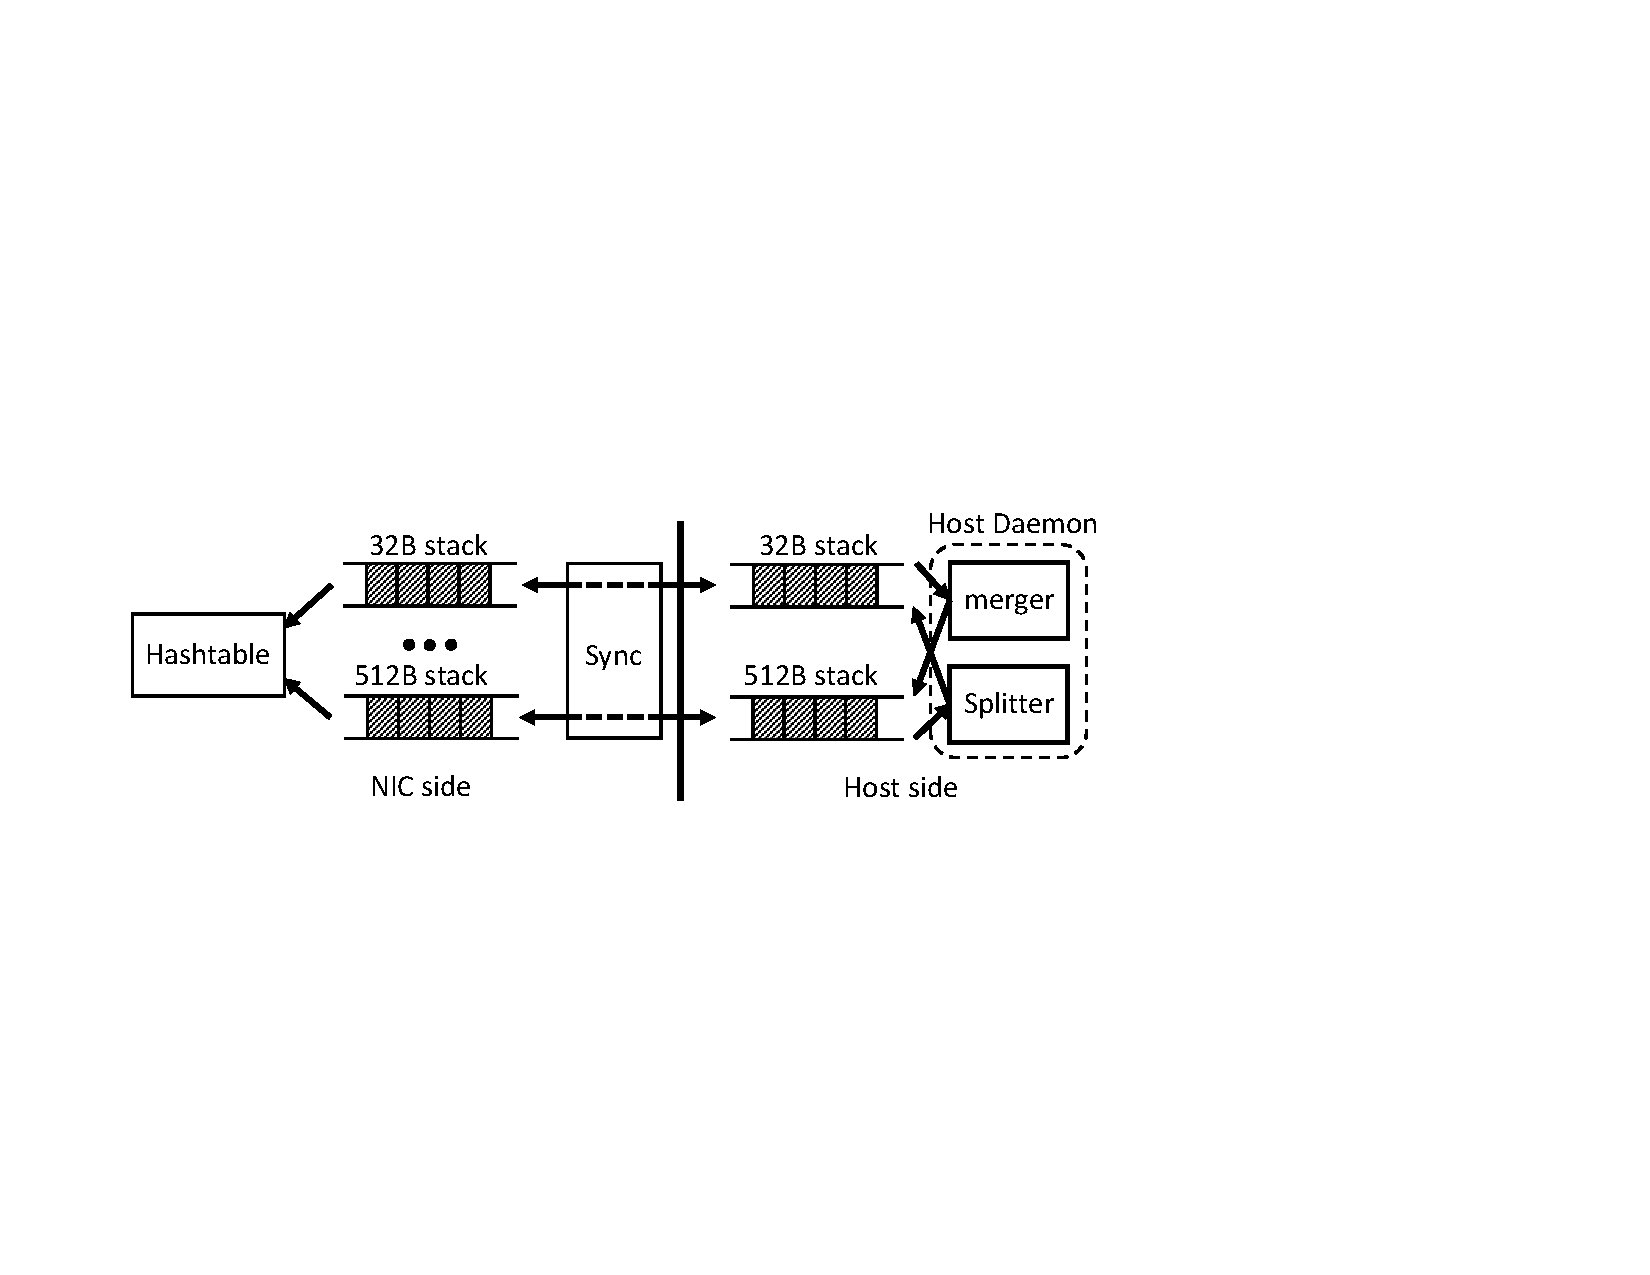
\includegraphics[width=.8\textwidth,page=1]{figure/cropped_slab.pdf}
	\caption{Slab memory allocator.}
	\label{kvdirect:fig:slab}
\end{figure}

As shown in Figure \ref {kvdirect:fig:slab}, for each slab size, the slab cache on the network card uses two double-end stacks to synchronize with the host DRAM. The left end of the network card's double-end stack (the left side in Figure \ref {kvdirect:fig:slab}) is popped by the allocator and pushed by the deallocator, and the right end synchronizes with the corresponding host end double-end stack via DMA. The network card monitors the size of the network card stack and synchronizes with the host stack according to the high watermark and low watermark. The host daemon periodically checks the size of the host end double-end stack. If it is higher than the high watermark, it triggers slab merging; if it is lower than the low watermark, it triggers slab splitting. Because each end of the double-end stack is exclusively accessed by either the network card or the host, and data is moved before moving the pointer, race conditions will not occur as long as the amount of data in the double-end stack is greater than the protection threshold.

\label{kvdirect:sec:slab-eval}

The communication overhead of the slab memory allocator comes from the network card accessing the available slab queue in the host memory. In this chapter, each slab entry is 5 bytes, the DMA granularity is 64 bytes, so the amortized DMA overhead for each slab operation is $5/64$ DMA operations. In addition, newly released slab slots on the network card can often be reused by subsequent allocation operations on the network card, so in many cases, no DMA operation is needed at all. To maintain a maximum throughput of 180M operations per second, in the worst case, 180M slab entries need to be transferred, consuming 720 MB/s PCIe throughput, which is 5% of the total PCIe throughput of the network card.

The computational overhead of the slab memory allocator comes from slab splitting and merging on the host CPU. Fortunately, they are not often called. For workloads with a stable key-value size distribution, newly released slab slots are reused by subsequent allocations, so they do not trigger splitting and merging.

Slab splitting requires moving continuous slab entries from one slab queue to another. When the workload switches from large key-values to small key-values, in the worst case, the CPU needs to move 90M slab entries per second, which only takes up 10% of the core, as it is just continuous memory copying.

Merging available slab entries into larger slab entries is a fairly time-consuming task, as this garbage collection process needs to fill the allocation bitmap with the addresses of slab entries, thus requiring random memory access. To sort the addresses of available slab entries and merge continuous slabs, radix sort \cite {satish2010fast} has better multi-core scalability than a simple bitmap. As shown in Figure \ref {kvdirect:fig:slab-garbage-collection}, merging all 4 billion free slab slots in a 16 GiB vector takes 30 seconds on a single CPU core, but only 1.8 seconds on 32 cores using radix sort \cite{satish2010fast}. Although garbage collection of free slab slots takes a few seconds, it runs in the background without stopping the slab allocator, and in fact only triggers when the workload switches from small key-values to large key-values.

\begin{figure}[t]
	\centering
	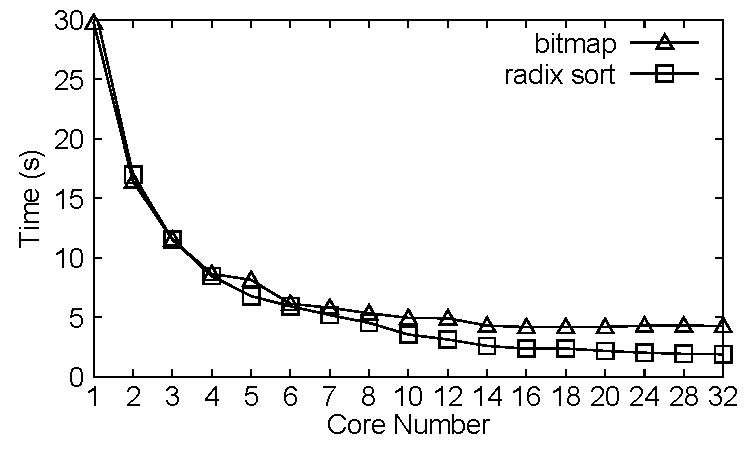
\includegraphics[width=0.6\textwidth]{slab-gc.pdf}
	\caption{Time overhead of merging 4 billion slab slots.}
	\label{kvdirect:fig:slab-garbage-collection}
\end{figure}

\subsection{Out-of-Order Execution Engine}
\label{kvdirect:sec:ooo}

In the key-value processor, the dependency between two key-value operations with the same key can lead to data hazards and pipeline stalls. This problem is more pronounced in single-key atomics, where all operations are dependent and must be processed one by one, limiting the throughput of atomic operations. This section borrows the concept of \textit{dynamic scheduling} from the field of computer architecture and implements a \textit{reservation station} to track all ongoing key-value operations and their \textit{execution contexts}.

To fully utilize PCIe, DRAM bandwidth, and processing pipelines, up to 256 concurrent key-value operations are needed. However, parallel comparison of 256 16-byte keys would occupy 40\% of the FPGA's logical resources. To avoid parallel comparison, this section stores key-value operations in a small hash table in on-chip BRAM, indexed by the hash of the key. Key-value operations with the same hash value are considered to have dependencies. Different keys may have the same hash value, so there may be false dependencies, but it will never miss dependencies. Key-value operations with the same hash are organized into a linked list structure, processed sequentially by the key-value processor. Hash collisions increase false dependencies and reduce key-value processing efficiency, so the reservation station includes 1024 hash slots, keeping the possibility of hash collisions below 25\%.

The reservation station not only saves operations temporarily suspended due to dependencies but also caches recently accessed key-values for \textit{data forwarding}. When the main processing pipeline completes a key-value operation, its result is returned to the client, and the latest value is forwarded to the reservation station. The reservation station checks pending operations in the same hash slot one by one, immediately executes operations with matching keys, and removes them from the reservation station. For atomic operations, calculations are performed in a dedicated execution engine. For write operations, the cached value is updated. The execution result is returned directly to the client. After scanning the dependency linked list, if the value cached in the reservation station has been updated, a PUT operation is issued to the main processing pipeline to write the cache back to the main memory. This data forwarding and fast execution path allows single-key atomic operations to process an operation per clock cycle\footnote{The clock frequency of the FPGA key-value processor in this chapter is 180 MHz, so the throughput can reach 180 M op/s.}, eliminating head-of-line blocking for frequently accessed keys. The reservation station ensures data consistency, as no two operations on the same key can proceed simultaneously in the main processing pipeline. Figure \ref{kvdirect:fig:ooo-mem-access} describes the structure of the out-of-order execution engine.

\begin{figure}[htbp]
	\centering
	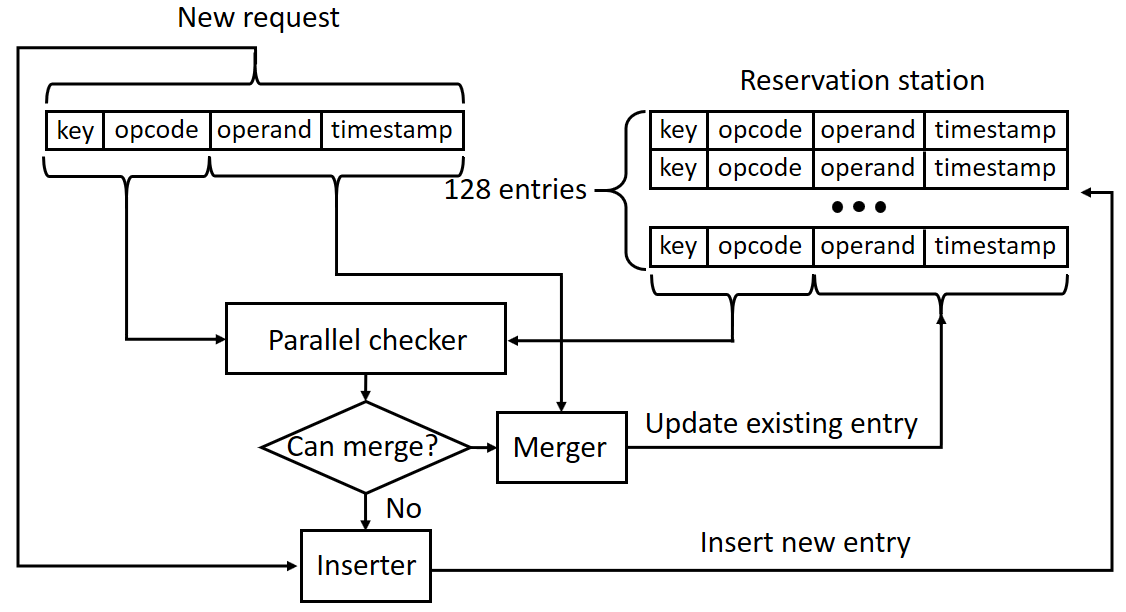
\includegraphics[width=.9\textwidth,page=1]{dynamic_scheduler.PNG}
	\caption{Out-of-order execution engine.}
	\label{kvdirect:fig:ooo-mem-access}
\end{figure}

\label{kvdirect:sec:ooo-eval}

The following evaluates the effectiveness of out-of-order execution. The workloads used include single-key atomics and long-tail distribution. The comparison method is a simple method that stalls the pipeline when a key conflict is encountered. The throughput of one-sided RDMA and two-sided RDMA \cite{kalia2016design} is used as a baseline.

\begin{figure}[htbp]
	\centering
	\subfloat[Atomic operations.\label{kvdirect:fig:ooo-atomic}]
	{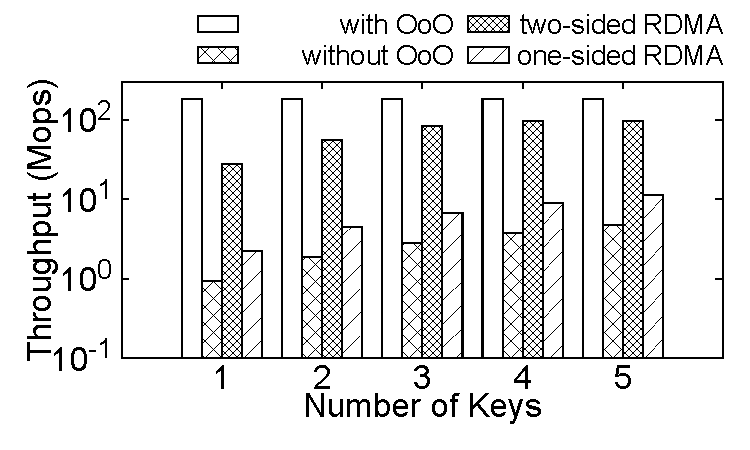
\includegraphics[width=.5\textwidth,page=1]{ooo_atomic.pdf}}
	\subfloat[Long-tail load.\label{kvdirect:fig:ooo-longtail}]
	{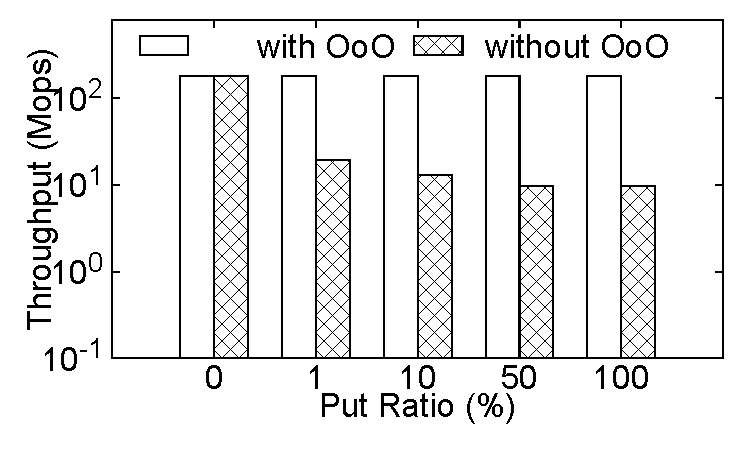
\includegraphics[width=.5\textwidth,page=1]{ooo_long-tail.pdf}}
	\caption{Efficiency of the out-of-order execution engine.}
	\label{kvdirect:fig:ooo-eval}
\end{figure}

Without the out-of-order execution engine, atomic operations have to wait for PCIe latency and processing latency in the network card, during which subsequent atomic operations on the same key cannot be executed. As shown in Figure \ref{kvdirect:fig:ooo-atomic}, the throughput of single-key atomic operations with the pipeline stalling method is 0.94~Mops, close to the 2.24~Mops measured using a commercial RDMA network card \cite{kalia2016design}. The higher throughput of the commercial RDMA network card can be attributed to its higher clock frequency and lower processing latency. With out-of-order execution, KV-Direct's single-key atomic operations can reach peak throughput, processing one key-value operation per clock cycle. In MICA \cite{lim2014mica}, the throughput of single-key atomics is limited by the processing capability of a single CPU core and cannot scale with multiple cores. In fact, the performance of atomic increment operations can scale with multiple cores \cite{kalia2016design}, but it relies on the commutativity between atomic operations, so it is not applicable to non-commutative atomic operations, such as compare-and-swap.

By utilizing out-of-order execution, the single-key atomic throughput has increased by 191 times, reaching the clock frequency limit of 180 Mops. When atomic operations are evenly distributed among multiple keys, the throughput of single-sided RDMA, double-sided RDMA, and KV-Direct without out-of-order execution grows linearly with the number of keys, but it still has a significant gap compared to the best throughput of KV-Direct using out-of-order execution.

Figure \ref {kvdirect:fig:ooo-longtail} shows the throughput under long-tail workloads. When a PUT operation finds any ongoing operation with the same key in the pipeline, the pipeline will pause. Long-tail workloads have multiple keys that are accessed very frequently, so two operations with the same key are likely to arrive almost simultaneously. When the proportion of PUT operations in all operations is higher, it is more likely that at least one of the two operations with the same key is a PUT operation, which triggers the pipeline to pause.

\subsection{DRAM Load Balancer}
\label{kvdirect:sec:dram-cache}

To further alleviate the burden of PCIe, this section schedules memory access between PCIe and the onboard DRAM of the network card. The network card DRAM has a capacity of 4 GiB and a throughput of 12.8 GB/s, which is an order of magnitude smaller than the key-value storage on the host DRAM (64 GiB) and slightly slower than the PCIe link (14 GB/s). One method is to put a fixed part of the key-value storage into the network card DRAM. However, the network card DRAM is too small to hold only a small part of the entire key-value storage. Another method is to use the network card DRAM as a cache for the host memory, but the throughput may even decrease due to the limited throughput of the network card DRAM (even lower than the PCIe throughput).

\begin{figure}[htbp]
	\centering
	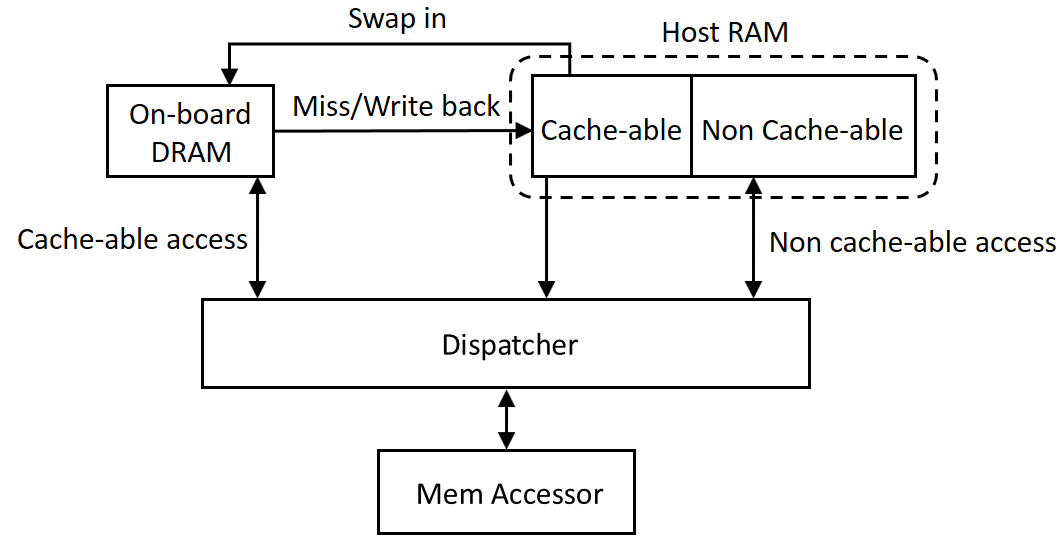
\includegraphics[width=0.8\textwidth,page=1]{load_balancer.PNG}
	\caption{DRAM load balancer.}
	\label{kvdirect:fig:cache}
\end{figure}

This section adopts a hybrid solution, using DRAM as a cache for a fixed part of the key-value storage in the host memory, as shown in Figure \ref {kvdirect:fig:cache}. The cacheable part is determined by the hash of the memory address, with a granularity of 64 bytes (DRAM memory access granularity). Choose a hash function so that the hash index and the address in the dynamically allocated memory have the same cache probability. The part of the cacheable memory in the entire key-value storage memory is called the \textit {load distribution ratio} ($ l $). If the load distribution ratio $ l $ increases, a larger proportion of the load will be allocated to the onboard DRAM, and the cache hit rate $h(l)$ will increase. To balance the load on PCIe and onboard DRAM, the load scheduling ratio $ l $ should be optimized so that:
$$\frac{l}{tput_{DRAM}} = \frac{(1-l) + l \cdot (1-h(l))}{tput_{PCIe}}$$

Specifically, under uniform load, let $k$ be the ratio of the size of the onboard DRAM to the size of the host key-value storage, then the cache hit rate $h(l) = \frac{\textnormal{cache size}}{\textnormal{cache-able memory size}} = \frac{k}{l}$. When $k \leq l$, the cache under uniform load is not efficient. Under long-tail load (Zipf distribution), let $n$ be the total number of key-values, then roughly $h(l) = \frac{\log (\textnormal{cache size})}{\log (\textnormal{cache-able part size})} = \frac{\log (kn)}{\log (ln)}$, when $k \leq l$. Under long-tail workloads, the cache hit probability of 1M cache in 1G key-value storage is as high as 0.7. The optimal $l$ can be obtained numerically, which will be discussed in section \ref{kvdirect:sec:different-nic}.

A technical challenge is to store metadata in the DRAM cache. For each cache line of 64 bytes, 4 address bits and a dirty flag bit of metadata are required. Because all key-value storage is accessed by the network card, no cache valid bit is needed. To store the 5 metadata bits of each cache line, if the cache line is expanded to 65 bytes, the DRAM performance will be reduced due to unaligned access; if the metadata is stored elsewhere, the number of memory accesses will double. Instead, this paper uses the spare bits in ECC (Error Correction Code) DRAM for metadata storage. ECC DRAM usually has 8 ECC bits for every 64 bits of data. In fact, to correct a one-bit error in 64 bits of data, only 7 additional check bits are needed. The 8th ECC bit is a parity bit used to detect double-bit errors. When accessing DRAM with a granularity of 64 bytes and in an aligned manner, each 64B data has 8 parity check bits. This paper increases the check granularity of parity from 64 data bits to 256 data bits, so double-bit errors can still be detected. This saves 6 additional bits that can be used to save address bits and dirty flag metadata.

Figure \ref {kvdirect:fig:cache-tput} shows the improvement in DRAM load scheduling throughput compared to using only PCIe. Under uniform workloads, the caching effect of DRAM can be ignored because its size is only 6% of the host key-value storage memory. Under long-tail workloads, about 30% of memory accesses are provided by DRAM cache. In general, in the case of 95% and 100% GET, the total throughput reaches the clock frequency limit of 180 Mops. However, if DRAM is simply used as a cache, the throughput will decrease because the DRAM throughput is lower than the PCIe throughput.

\begin{figure}[htbp]
	\centering
	{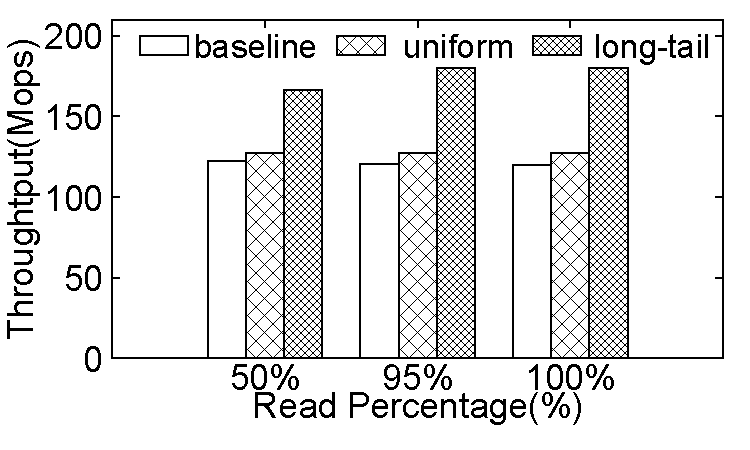
\includegraphics[width=.5\textwidth,page=1]{load_balancer.pdf}}
	\caption{DMA throughput under load distribution (fixed load distribution ratio at 0.5).}
	\label{kvdirect:fig:cache-tput}
\end{figure}

\subsection{Vector Operation Decoder}

The entire key-value processor design views batch processing as a general principle.
This includes batch fetching multiple hash slots in a bucket, batch synchronization of idle slab queues with host memory, lazy slab splitting and merging, and reservation stations batch processing dependent key-value operations along the linked list.
Batch processing improves performance by spreading control plane overhead across multiple effective data plane payloads.

Compared to PCIe, the network is a more scarce resource, with lower bandwidth (5~GB / s) and higher latency (2~$\mu$s).
Ethernet RDMA write packets have 88 bytes of header and padding overhead, while PCIe TLP packets only have 26 bytes of overhead.
This is why previous FPGA-based key-value stores \cite{blott13hotcloud,blott2015scaling} did not saturate PCIe bandwidth, despite their hash table design being less efficient than KV-Direct.
To fully utilize network bandwidth, \textit {client batching} is required in two aspects: batch processing multiple key-value operations in a single packet, and supporting vector operations for more compact representation. For this, a decoder is implemented in the key-value engine to decompress multiple key-value operations from a single RDMA packet.
Observing that many key-values have the same size or repeated values, the key-value format includes two flag bits to allow copying key and value sizes, or values of previous key-values in the packet.
Fortunately, many important workloads (\textit {such as graph traversal, parameter servers}) can be batched for key-value operations.
Looking forward, if higher bandwidth networks can be used, batching will not be necessary.

To evaluate the efficiency of vector operations in KV-Direct,
Table \ref {kvdirect:tab:vec_throughput} compares the throughput of atomic vector increments with two alternatives:
(1) If each element is stored as a different key, the bottleneck is the network transmitting key-value operations.
(2) If the entire vector is stored as a large opaque value, retrieved and processed by the client, the overhead of sending the vector over the network is also high.
In addition, the two alternatives in Table \ref {kvdirect:tab:vec_throughput} cannot ensure consistency within the vector when accessed by multiple clients simultaneously. Adding synchronization between clients would incur further overhead.

\begin{table}[htbp]
	\centering
	\caption{Throughput of vector operations (GB/s).}
	\label{kvdirect:tab:vec_throughput}
	\small
		\begin{tabular}{|l|r|r|r|r|r|}
			\hline
			Vector size (bytes)              & 64    & 128   & 256   & 512   & 1024  \\ \hline
			Vector update (with return)    & 11.52 & 11.52 & 11.52 & 11.52 & 11.52 \\ \hline
			Vector update (no return) & 4.37  & 4.53  & 4.62  & 4.66  & 4.68  \\ \hline
			Each element a key         & 2.09  & 2.09  & 2.09  & 2.09  & 2.09  \\ \hline
			Retrieve for client processing             & 0.03  & 0.06  & 0.12  & 0.24  & 0.46  \\ \hline
		\end{tabular}
\end{table}

KV-Direct clients package key-value operations in network packets to reduce packet header overhead.
Figure \ref {kvdirect:fig:eval-network-batching} shows that network batching can increase network throughput by 4 times, while keeping network latency below 3.5~$\mu$s.

\begin{figure}[htbp]
	\centering
	\subfloat[Throughput.\label{kvdirect:fig:network-batching-bw}]
	{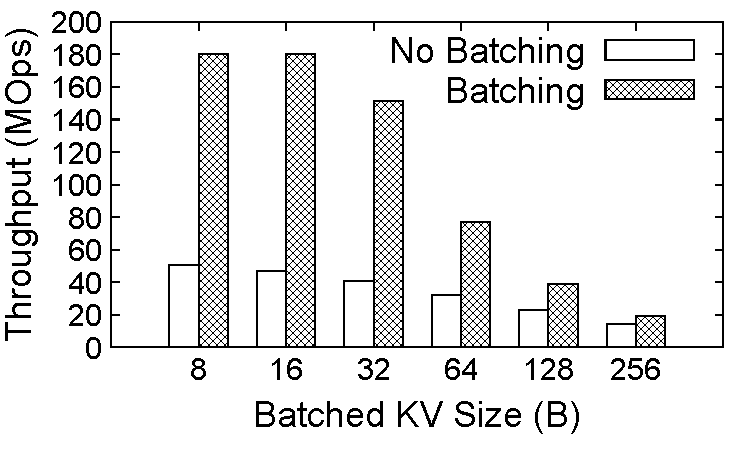
\includegraphics[width=.5\textwidth,page=1]{net_batching_bw.pdf}}
	\subfloat[Latency.\label{kvdirect:fig:network-batching-lat}]
	{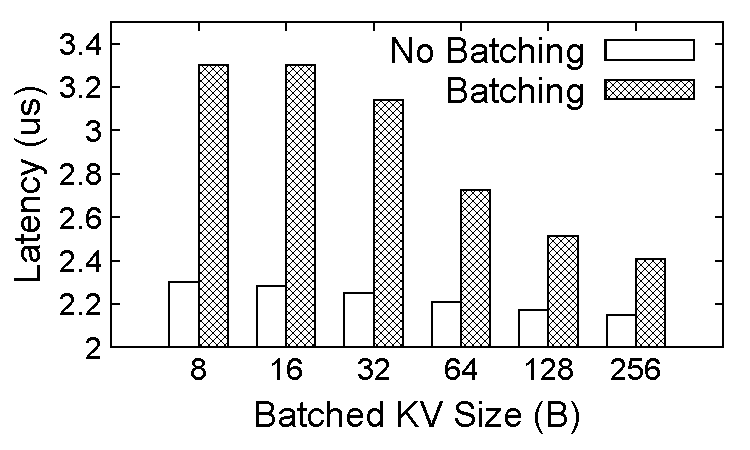
\includegraphics[width=.5\textwidth,page=1]{net_batching_lat.pdf}}
	\caption{Efficiency of network batching.}
	\label{kvdirect:fig:eval-network-batching}
\end{figure}

\egg{
\subsubsection{Congestion Avoidance}
\label{kvdirect:sec:congestion-avoidance}

In addition to throughput, another important factor is latency.
From the client's perspective, the key-value processor is a path with multiple bottlenecks and buffers, \eg, PCIe and DRAM access.
If all buffers in the key-value processor are filled up, the GET latency would exceed 10~$\mu$s.
To mitigate the bufferbloat problem, we implement a congestion avoidance logic to limit the number of in-flight key-value operations \textit{inside the key-value processor}.
The key-value processor maintains a \textit{key-value operation window} and leverages credit-based flow control mechanism in RDMA to back-pressure key-value storage clients.
To adapt key-value operation window size to the workload, we measure the running average of key-value processing delay and adjust the window size according to TCP Vegas congestion avoidance algorithm~\cite{brakmo1995tcp}.
%We use delay as the congestion signal instead of ECN, because the queues whose sizes are hard to measure.
}
